%!TEX root = ../main.tex
\chapter{Diseño del sistema de control}

\section{Modelo matemático del sistema}

\subsection{Subsistema mecánico}

{\parindent0pt
Este subsistema está compuesto por el eje de baja velocidad, el cual está conectado al rotor, el eje de alta velocidad 
y la caja de engranes (\emph{gearbox}). Estos tres componentes juntos conforman el tren motriz de la turbina eólica 
\cite{soltani2013}. La caja de engranes tiene como principal objetivo convertir la velocidad rotacional baja proveniente 
del rotor a una velocidad rotacional mayor requerida por el generador. Es importante destacar que la caja de engranes 
de una turbina eólica tiene una relación de engranes fija y no variable (como las que se encuentran en los automóviles) 
dado que su función únicamente es generar una mayor velocidad rotacional para alimentar al generador.
\\

Permitir que el rotor gire a mayor velocidad ayudaría a tener una transmisión con una menor relación de engranes, 
lo cual es beneficioso considerando que se trata de uno de los componentes más costosos en la turbina; sin embargo, 
esto conlleva a mayor estrés mecánico y eléctrico en el resto de los componentes, por lo que una disminución en esta 
relación de engranes debe hacerse con cuidado \cite{Burton2011}.
\\

En \cite{soltani2013} se presenta un modelo matemático para este subsistema en el cual se considera: 1) el eje de baja 
velocidad compuesto por un momento de inercia rotacional ($J_r$), un amortiguador viscoso y un resorte rotacional con 
amortiguación viscosa; 2) la caja de engranes perfectamente rígida (se asume que su flexibilidad es transferida a través 
de la deformación del eje de baja velocidad); y 3) el eje de alta velocidad compuesto por una inercia ($J_g$) y un amortiguador ($B_g$).
El modelo dinámico de esta configuración se puede simplificar a partir de incluir un modelo simplificado del tren 
motriz. La dinámica completa del sistema está dada por:

\begin{equation}
    J_t \dot{\omega}_r = \frac{1}{N_g}T_r - T_g - T_\ell
    \label{eq:torque_balance_complete}
\end{equation}

donde $J_t$ es el momento de inercia combinado del rotor y generador, $N_g$ es la relación de la caja de engranes, $T_r$ 
es el par aerodinámico recibido por el viento, $T_g$ es el par eléctrico que recibe el generador y $T_\ell$ representa el par de pérdidas.
Una forma adicional de representar la dinámica del sistema es con la ecuación:

\begin{equation}
    J \dot{\omega}_m = -f \omega_m + T_m - T_e
    \label{eq:torque_balance_simplified}
\end{equation}

donde $\omega_m$ representa la velocidad angular, $f$ es el coeficiente de fricción viscosa, $T_m$ es el par mecánico 
y $T_e$ el par eléctrico. La equivalencia se da al considerar que $T_m = T_r/N_g$, $T_e = T_g$ y que el término 
$f\omega_m$ modela las pérdidas mecánicas representadas por $T_\ell$ en la ecuación anterior.
En adelante, se utilizará la versión simplificada del balance de torques (\ref{eq:torque_balance_simplified}) 
puesto que permite manejar el torque de pérdidas como un valor constante en la dinámica del sistema.
\\

Es importante aclarar que en la práctica la potencia real que se puede obtener del viento es limitada y, por 
tanto, también lo es el torque aerodinámico/mecánico. En particular, la potencia extraída del viento está dada por
\footnote{Esta es una ecuación fundamental en aerodinámica de turbinas eólicas, ampliamente documentada en 
la literatura. Para una derivación detallada véase Burton et al. \cite{Burton2011}. Para aplicaciones prácticas 
y consideraciones de diseño véase Hau \cite{Hau2013}.}:
\begin{equation}
    P_a = \frac{1}{2}\rho \pi r^2 v_w^3 C_p(\lambda,\beta)
    \label{eq:aerodynamic_power}
\end{equation}

donde $\rho$ es la densidad del aire, $r$ es el radio de giro de las aspas, $v_w$ la velocidad del viento y 
$C_p(\lambda,\beta)$ es el coeficiente de potencia en términos de la relación de velocidad punta ($\lambda$) y el angulo de ataque de las aspas ($\beta$).
\\

La potencia se relaciona directamente con el torque aerodinámico mediante la ecuación:
\begin{equation}
    T_r = \frac{P_a}{\omega_r}
    \label{eq:aerodynamic_torque}
\end{equation}

En (\ref{eq:torque_balance_simplified}) utilizamos una versión simplificada del balance de torques. 
En esta ecuación se define cada torque como sigue:

\begin{equation}
    T_m = r\frac{\kappa_1}{v_w} \frac{C_p(\lambda,\beta)}{\lambda}
    \label{eq:mechanical_torque}
\end{equation}

\begin{equation}
    T_e = \frac{3}{2}p\phi i_q
    \label{eq:electrical_torque}
\end{equation}

Estas ecuaciones introducen las variables $\kappa_1$, la cual es un parámetro de diseño y un valor 
constante en la simulación, el flujo eléctrico en el generador ($\phi$) y la corriente en el eje de 
cuadratura del generador ($i_q$). Estas últimas dos variables serán tratadas
a profundidad en la sección del subsistema eléctrico.



\subsection{Coeficiente de potencia}

Durante su operación, el rotor de la turbina eólica absorbe energía de la corriente de aire, 
lo cual promueve su movimiento. El poder de absorción y las condiciones de operación del aerogenerador dependen, por tanto, 
del área efectiva de barrido ($A_R$), la velocidad del viento y los cambios que ocurren en estas 
cantidades en el campo de flujo del rotor. Durante el proceso de extracción de la potencia el flujo de aire experimenta
desaceleración axial, una desviación tangencial al momento de chocar con el área del rotor y una 
expansión del área de la sección transversal una vez que ha pasado el rotor (efecto estela) \cite{heier2014}.
\\

La potencia teórica extraida por la turbina se puede expresar como:

\begin{align}
    P_W = A_R\frac{\rho}{2}v^3
    \label{eq:theoretical_power}
\end{align}

y de acuerdo con Betz \cite{betz1926}, la potencia máxima teórica extraida sería:

\begin{align}
    P_{W_{\text{max}}} = \frac{16}{27}A_R\frac{\rho}{2}v_1^3 
    \label{eq:max_theoretical_power}
\end{align}

donde $v_1$ es la velocidad del viento antes del rotor.
\\

El cociente entre la potencia teórica extraida y la potencia en la masa de aire en movimiento, la cual se expresa como:

\begin{align}
    P_0 = A_R\frac{\rho}{2}v_1^3
\end{align}

define el coeficiente de potencia (también llamado coeficiente de rendimiento):

\begin{align}
    c_p = \frac{P_W}{P_0}
\end{align}

Se puede observar que el coeficiente de potencia consiste en el cociente entre el cubo la velocidad $v$ 
(el cual es una función de las velocidades $v_1$, $v_2$ y $v_3$, siendo estas las velocidades antes, en 
y después del rotor, respectivamente), y el cubo de la velocidad del viento antes del rotor ($v_1$). En 
la práctica, la manera más común de obtener este valor es utilizando métodos 
computacionales y artificios matemáticos más complejos (se puede encontrar un desarrollo detallado del 
método \emph{blade element} en \cite{heier2014}).
\\

Un punto importante a notar es que, de acuerdo con \cite{Burton2011}, en turbinas modernas de tres palas 
el valor máximo de $C_P$ es de solo 0.47, lo cual se aleja considerablemente del límite teórico de Betz, 
y se logra con un valor de la 
relación de velocidad punta de $\lambda^\star \approx 7$. Esto se puede ver más fácilmente en las curvas 
$C_P - \lambda$ (vease figura \ref{fig:Cp_vs_lambda}). 
\begin{figure}
    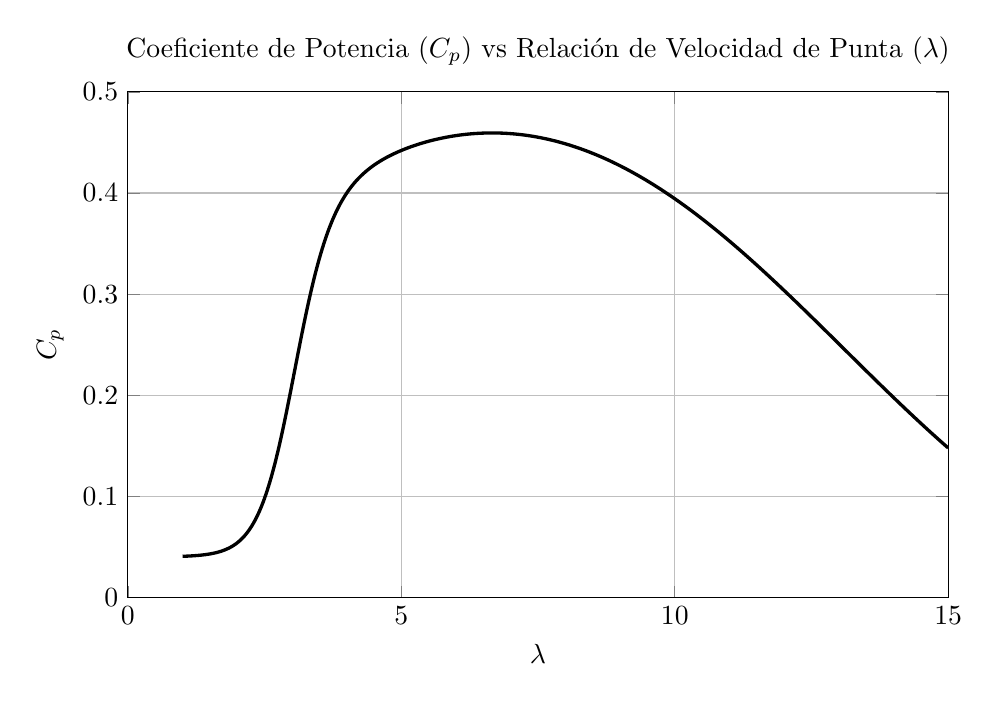
\begin{tikzpicture}
    \begin{axis}[
        title={Coeficiente de Potencia ($C_p$) vs Relación de Velocidad de Punta ($\lambda$)},
        xlabel={$\lambda$},
        ylabel={$C_p$},
        xmin=0, xmax=15,
        ymin=0, ymax=0.5,
        %xtick={0,1,2,3,4,5,6,7,8,9,10,11,12,13,14,15},
        xtick={0,5,10,15},
        ytick={0,0.1,0.2,0.3,0.4,0.5},
        grid=both,
        minor grid style={gray!25},
        major grid style={gray!50},
        width=12cm,
        height=8cm,
        every axis plot/.append style={very thick}
    ]
    
    % Definir la curva ajustada para alcanzar el máximo en lambda=7, Cp=0.47
    \addplot[smooth, domain=1:15, samples=200] {
        0.47 * (1/(1 + exp(-3*(x-3)))) * (1/(1 + 0.15*exp(0.3*(x-8)))) * (1-0.01*(x-8)^2) + 0.04
    };
    
    \end{axis}
    \end{tikzpicture}
    \caption{Curva de $\lambda$ vs $C_p$. Adaptada de \cite{Burton2011}}
    \label{fig:Cp_vs_lambda}
\end{figure}
\\


Con el objetivo de obtener un valor del coeficiente de potencia ajustado a los parámetros utilizados durante el modelado de la turbina se utilizará una aproximación mediante una función analítica de $c_p$.
En \cite{man1981} se desarrolla una expresión para el coeficiente de potencia como la siguiente función de la relación de velocidad punta y el angulo de inclinación de las palas:

\begin{align}
    C_p = c_1 \left( c_2 - c_3\vartheta - c_4\vartheta^x - c_5 \right) e^{-c_6(\lambda,\vartheta)}
\end{align}

Los valores de las constantes cambian según el método y modelo utilizado. A partir del procedimiento en \cite{amlang1992}, los valores de estas constantes se definen como:
\begin{align}
    \begin{array}{lll}
        c_1 = 0.5, &c_2 = \frac{116}{\lambda_i}, &c_3 = 0.4,
        \\
        c_4 = 0, &c_5 = 5, &c_6 = \frac{21}{\lambda_i}
    \end{array}
\end{align}

y
\begin{align}
    \frac{1}{\lambda_i} = \frac{1}{\lambda + 0.08\vartheta} - \frac{0.035}{\vartheta^3 + 1}
\end{align}

$\vartheta$ es el angulo de inclinación (\emph{pitch}) de las palas.

\emph{TODO: agregar el valor de x según lo que se haya usado en la simulación.}

\subsection{Subsistema eléctrico}

La parte eléctrica del modelo está compuesta por: 1) el generador eléctrico (PMSG), 2) la electrónica de potencia y 3) la carga que será alimentada. La elección del generador 
eléctrico depende de factores como la potencia requerida para ser extraída del viento, la eficiencia requerida, la cantidad de mantenimiento requerida, la fiabilidad y la 
longevidad del generador en comparación con el resto de los componentes y la vida útil general de la turbina, entre otros. 
\\

Dos de los tipos de generadores eléctricos más usados en WECS son los Generadores de Inducción Doblemente Alimentados (DFIG, por sus siglas en inglés: \emph{Doubly-Fed Induction Generator}) 
y los Generadores Síncronos de Imanes Permanentes (PMSG por sus siglas en inglés: \emph{Permament Magnent Synchronous Generator}). Por un lado, los generadores tipo DFIG, como 
su nombre lo indica, presentan una doble alimentación de voltaje hacia el rotor y el estator. Este último puede ser 
conectado directamente a la red y al rotor a través de un convertidor \cite{dahiya2019}. Este tipo de generadores es el más usado en turbinas eólicas de velocidad variable
\cite{dahiya2019,soltani2013}.
Los PMSG, por su parte, tienen la característica de permitir el accionamiento 
directo (\emph{direct drive}) del generador, lo cual hace posible la eliminación del \emph{gearbox} de la mecánica del sistema. Esto se logra a partir de incluir un alto número 
de polos en el diseño del generador, lo que permite la operación a bajas velocidades del rotor \cite{soltani2013, swibki2020}.
\\

Dentro de las consideraciones generales de ambos generadores al momento de decidir entre uno u otro se debe mencionar: i) la mayor eficiencia de los PMSG al operar efectivamente 
en un rango más amplio de condiciones climáticas (los DFIG operan con mayor eficiencia a velocidades altas del viento), ii) los costos de construcción asociados a los PMSG, 
en particular por los materiales utilizados en su fabricación; y iii) la necesidad de una caja de cambios en los DFIG, lo que incrementa su costo e introduce el problema del 
desgaste de estos componentes con el tiempo, así como la necesidad de mantenimiento a los componentes. 
Ambos tipos de generadores están diseñados  para operar a velocidad variables y permiten el control de 
la potencia reactiva \cite{dahiya2019, swibki2020,Lei2006,feijoo2000}. 
\\

Las ecuaciones dinámicas son similares en ambos 
tipos de generadores como se puede ver en \cite{Lei2006} para DFIG y en \cite{cisneros2020} para PMSG. 
Las diferencias se dan principalmente en que DFIG se incluyen también los voltajes del rotor además del estator \cite{Lei2006}.
El posterior desarrollo matemático en esta tesis asume la elección de un Generador Síncrono de Imanes 
Permanentes (PMSG).
\\

Los generadores son sistemas eléctricos trifásicos en los que cada señal de voltaje, intensidad de corriente 
o flujo magnético se encuentra desfasada $120^\circ$ con respecto a la anterior. En este sentido, a cada fase se le 
asigna una letra para denotar sus respectivas magnitudes. Este sistema se conoce como el \textbf{marco de referencia}
\emph{abc}. A pesar de que este marco de referencia emplea las variables físicas reales del sistema ($v_{abc}$, $i_{abc}$ y $\phi_{abc}$), 
introduce una mayor complejidad al momento de diseñar el control debido a la existencia de términos dependientes del 
tiempo y cuyo comportamiendo suele ser senoidal. 
\\

Para simplificar el análisis matemático y el diseño del control se utiliza un cambio de variable que permite transformar 
las variables del sistema del marco de referencia \emph{abc} a un nuevo marco de referencia \emph{dq0} (en lo sucesivo nos referiremos 
únicamente a este marco de referencia como \emph{dq} o coordenadas \emph{dq}). En \cite{krause2013} este cambio de variable se maneja como
una transformación a un \textbf{marco de referencia arbitrario}, la cuál podría considerarse una versión genérica que agrupa a las trasformadas
específicas de Park \cite{park1929} para distintas aplicaciones. En particular, el cambio del marco de referencia \emph{abc} a \emph{dq} implica el uso de 
las transformadas de Clarke \cite{clarke1943} y Park de manera sucesiva. 
\\

En el nuevo marco de referencia las variablas de tipo \emph{dq} se conocen como variables del \textbf{eje directo} para \emph{d} y variables 
del \textbf{eje de cuadratura} para \emph{q}. Las variables \emph{0's} no serán incluidas ya que dichas magnitudes están aritméticamente relacionadas
con las variables \emph{abc} y solo se incluiran aquellas que permitan condiciones de balance. i.e. \emph{dq} al ser independientes del tiempo \cite{krause2013,krause1998}.
\\

El análisis dinámico del generador de la turbina parte de leyes fundamentales de la electricidad
\footnote{El desarrollo completo de las ecuaciones dinámicas del sistema se puede encontrar en \cite{krause2013}}. 
En particular, para los \textbf{componentes resistivos} 
del generador, la ley de Ohm establece que:
\begin{align}
    v_{abc} = R_s i_{abc}
\end{align}

donde $R_s$ es la matriz de resistencias del estator. Al transformar esta relación al marco de referencia arbitrario obtenemos:
\begin{align}
    v_{dq0} = K_sR_s(K_s)^{-1} i_{dq0}
\end{align}

Asumiendo que cada uno de los embobinados de fase del estator tienen la misma resistencia se cumple entonces que:
\begin{align}
    K_sR_s(K_s)^{-1} = R
\end{align}

Resultando en la siguiente expresión para el voltaje:
\begin{align}
    v_{dq} = R i_{dq}
\end{align}

Por su parte, los \textbf{elementos inductivos} siguen la ley de inducción electromagnética de Faraday,
\begin{align}
    v_{abc} = \frac{d}{dt}\lambda_{abc}
\end{align}

donde $\lambda_{abc}$ son los enlaces de flujo, los cuales a su vez representan el 
flujo magnético total que atraviesa un embobinado y que, en el caso de un PMSG, recibe dos aportaciones principalmente:
el flujo magnético generado en los devanados del estator y el flujo producido en los imanes permanentes en el rotor.
Al transformar coordenadas \emph{dq} obtenemos:
\begin{align}
    v_{dq} = \omega\lambda_{dq} + \frac{d}{dt}\lambda_{dq}
\end{align}

La expresión final de los voltajes \emph{dq} resulta de la suma de los voltajes de los elementos resistivos e inductivos. 
Por tanto,
\begin{align}
    v_{dq} = Ri_{dq} + \omega\lambda_{dq} + \frac{d}{dt}\lambda_{dq}
\end{align}

En \cite{krause2013} los valores de $\lambda_{dq}$ se asignan como sigue. 
\begin{align}
    &\lambda_q = L_q i_q
    \\ 
    &\lambda_d = L_d i_d + \lambda_m
\end{align}

donde $L_q = L_{ls} + L_{mq}$, $L_d = L_{ls} + L_{md}$. i.e. en ambos casos, la inductancia total de cada eje es la suma de la inductancia
de fuga más la inductancia de magnetización (inducida por los imanes permanentes); $\lambda_m$ es el enlace de flujo de los imanes permanentes.
\\

Una manipulación algebráica permite llegar a las siguientes ecuaciones dinámicas que caracterizan el funcionamiento 
del generador utilzando coordenadas \emph{dq}:


\begin{equation}
    \begin{aligned}
        L\frac{di_q}{dt} &= -Ri_d + pLi_q\omega_m - v_d
        \\
        L\frac{di_d}{dt} &= -Ri_q - pLi_d\omega_e + p\phi\omega_e - v_q 
    \end{aligned}
    \label{eq:electrical_subsystem}
\end{equation}

donde $i_d$, $i_q$, $v_d$ y $v_q$ son los voltajes y corrientes en el eje directo y de cuadratura, $p$ es el número de polos,
$\phi$ es el flujo magnético en el generador y $R$ es el valor de la resistencia en el generador. 

\subsection{Sistema acoplado}

A partir de las ecuaciones del subsistema mecánico (\ref{eq:torque_balance_simplified}) y el subsistema eléctrico (\ref{eq:electrical_subsystem}) 
obtenemos el modelo dinámico que define el comportamiento del sistema completo de la turbina eólica:

\begin{align}
    L\frac{di_q}{dt} &= -Ri_d + pLi_q\omega_m - v_d
    \\
    L\frac{di_d}{dt} &= -Ri_q - pLi_d\omega_e + p\phi\omega_e - v_q 
    \\
    J \dot{\omega}_m &= -f \omega_m + T_m - T_e
    \label{eq:full_system}
\end{align}

Donde
\begin{align}
    T_m &= r\frac{\kappa_1}{v_w} \frac{C_p(\lambda,\beta)}{\lambda}
    \\
    T_e &= \frac{3}{2}p\phi i_q
    \\
    \lambda &= \frac{r\omega_m}{v_w}
\end{align}

Los voltajes $v_d$ y $v_q$ se pueden manipular de forma libre, es decir, corresponden a las variables de control.

\section{Diseño del control de torque}

\subsection{Objetivos de control}

En turbinas éolicas de velocidad variable obtenemos una mayor eficiencia del sistema al reducir las pérdidas
del generador para una carga dada. Dentro del marco de referencia \emph{dq} la corriente $i_q$ se emplea para
inducir el torque en el generador. Esto se puede apreciar en la ecuación del torque eléctrico (\ref{eq:electrical_torque})
en la cual la corriente $i_d$ no tiene ninguna contribución. Por lo anterior, y para minimizar pérdidas, 
buscamos llevar la corriente del eje directo a un valor de $i_d = 0$ \cite{chinchilla2006}.
Por su parte, el valor de la corriente $i_q$ deberá ser controlado con el objetivo de maximizar la extracción 
de potencia del viento. Lo anterior tiene como objetivo final la regulación de la velocidad rotacional del 
rotor de la turbina. 
\\

Previamente se introdujo el coeficiente de potencia. En dicha función se cumple que
para cada velocidad del viento existe una velocidad angular óptima que maximiza $C_p(\lambda,\beta)$ \cite{Leidhold2002,nak2013}.
Dicha velocidad angular óptima se conoce como \textbf{punto de máxima potencia} o MPP (por sus siglas en inglés: 
\emph{Maximum Power Point}) y al método o estrategia de control para encontrar este punto se le conoce como
\textbf{seguimiento del punto de máxima potencia} o MPPT (Por sus siglas en inglés: \emph{Maximum
Power Point Tracking}). Aunque existen varios métodos para el MPPT, en \cite{nak2013} se 
clasifican en tres principales categorías: control de la relación de velocidad punta (TSR), búsqueda 
\emph{Hill-climbing} (HCS), también conocida como \emph{Perturb \& Observe} (P\&O); y, por último, control de 
retroalimentación de la señal de potencia (PSF).
\\

Se considerará en el diseño del control del torque un algoritmo P\&O (o HCS) para el control de la velocidad óptima del
rotor. La estrategia principal en este tipo de control consiste en tomar muestras de la salida de potencia 
continuamente y compararlas con la salida inmediata anterior. Dependiendo de si la salida actual es mayor o menor
se incrementa o decremente el torque eléctrico del generador \cite{wang2004,buehring1981}.
\\

Una de las ventajas que ofrece un algoritmo HCS consiste en ser, de entre los tres tipos de estrategias
de control, el único que no requiere un conocimiento previo del sistema WECS y que es independiente de 
las características del viento, del generador y de la turbina en general. Lo anterior implica que el MPPT
se puede realizar en conjunto con otras estrategias de control para WECS como el \emph{pitch control} 
\cite{kazmi2011}. 
\\

Por otra parte, los algoritmos HCS presentan dos desventajas que pueden estar inducidas por alteraciones 
en la velocidad del viento en periodos cortos de tiempo o a un tamaño de paso del algoritmo inadecuado 
\cite{kazmi2011,xia2013}. Sin ambargo, estos problemas serán tratados con mayor detalle en la sección de
simulación dado que, como se mencionó, su Implementación es independiente de la dinámica del generador y 
del resto de la turbina. 
\\

Por tanto, los objetivos de control se pueden resumir en:
\begin{enumerate}
    \item regular la corriente del eje directo en $i_d = i_d^\star = 0$ para minimizar pérdidas,
    \item regular la velocidad angular $\omega_m$ a un valor constante positivo que corresponta a 
        la velocidad óptima del MPPT.
\end{enumerate}

\subsection{Estrategia de control}

El sistema de control propuesto combina distintas estrategias para regulación de la velocidad del rotor.
Para empezar, se regula el torque del generador mediante un control PI cuyo objetivo es mantener las variables
del PMSG en coordenadas \emph{dq} en un régimen adecuado para la máxima extracción de potencia del viento. Para
esto, se utiliza como referencia el valor de la velocidad rotacional y un algoritmo de seguimiento del punto de
máxima potencia (MPPT) para ajustar la velocidad rotacional óptima a la cual se quiere seguir.
\\

Con base en la sección anterior, en particular las ecuaciones (\ref{eq:full_system}) que describen el 
sistema completo, nos interesa encontrar las ecuaciones que definen las variables de control $v_d$ y 
$v_q$. La estrategia utilizada para lograr esto es buscar un patrón de ``cancelación'' de términos 
no lineales combinado con la inserción de términos del control PI. De este modo, partiendo del modelo 
dinámico, se tiene para $v_d$:
\begin{align}
    v_d = pL i_q \omega_m + u_{\tt pi}^d \label{valUd},
\end{align}

donde $u^d_{\tt pi}$ es la salida del controlador PI definida, por tanto, como:
\begin{equation}
\begin{aligned}
    u_{\tt pi}^d &= k_{P1}(i_d-i_{d}^{\star}) + k_{I1}\xi_1\\
    &=k_{P1}i_d + k_{I1}\xi_1\\
    \dot{\xi_1} &= i_d-i_d^{\star}= i_d.
\end{aligned}
\label{eqUd}
\end{equation}

De manera similar para $v_q$:
\begin{align}
v_q = -pL i_d \omega_m + p\phi \omega_m + u_{\tt pi }^q,
\label{eqnVq}
\end{align}

donde $u_{\tt pi}^q$ corresponde al controlador PI definido por las siguientes ecuaciones:
\begin{equation}
\begin{aligned}
u^q_{\tt pi} &= k_{P2}(i_q - i_{q}^{ref}) + k_{I2}\xi_2 \\
\dot{\xi}_2 &= i_q - i_{q}^{ref},
\end{aligned}
\label{PI2}
\end{equation}

con la señal $i_q^{ref}$ definida como :
\begin{equation}\label{xi}
\begin{aligned}
i_{q}^{ref} &= k_{P3}(\omega_m - \omega_m^\star) + k_{I3}\xi_3 \\
\dot{\xi}_3 &= \omega_m - \omega_m^\star.
\end{aligned}
%\label{PI3}
\end{equation}

La estructura completa del control está definida por tres lazos de retroalimentación caracterizados
como sigue:

\begin{enumerate}
    \item \textbf{control de la corriente $i_d$}: \begin{itemize}
        \item entrada: la corriente $i_d$ medida que se busca mantener en 0,
        \item salida: el valor de $u_d$ para que $v_d$ compense las variaciones en $i_d$;
    \end{itemize}
    \item \textbf{control de la corriente $i_q$}: \begin{itemize}
        \item entrada: error de la corriente en el eje de cuadratura $(i_q - i_q^{ref})$,
        \item salida: el valor de $u_q$ para $v_q$;
    \end{itemize}
    \item \textbf{control de velocidad}: \begin{itemize}
        \item entrada: el error de la velocidad del rotor $(\omega_m - \omega_m^\star)$;
        \item salida: la señal de referencia de la corriente $i_q^{ref}$.
    \end{itemize}
\end{enumerate}

La sustitución de \eqref{eqUd} en \eqref{valUd} y, la sustitución de la expresión resultante en la primera
ecuación de \eqref{eq:electrical_subsystem} da lugar a las ecuaciones de $\Sigma_1$. Esto es:
\begin{align}
    L\dot{i_d} &= -(R+k_{P1})i_d - k_{I1}\xi_1\\
    \dot{\xi_1} &= i_d,
\end{align}

o, equivalentemente, en representación de estados,
\begin{align}
    \mathbf{\Sigma_1:}\;\;\: \dot x= & \underbrace{\begin{bmatrix}0&1\\  -\frac{1}{L}k_{I1} & -\frac{1}{L}(R+k_{P1}) 
    \end{bmatrix}}_{A_1}x
 \end{align}

 con $x=\mathrm{col}(\xi_1,i_d)$. Claramente este subsistema corresponde a un sistema lineal e invariante en 
 el tiempo, completamente desacoplado de la dinámica de $\omega_m$ e $i_q$. Adicionalmente, el polinomio característico 
 de  $A_1$ es el siguiente:
 \begin{align}\label{p1}
 p_1(s)=s^2 + \frac{k_{P1}+R}{L}s + \frac{k_{I1}}{L}.
 \end{align}

 Luego, por el criterio de estabilida de Routh, la condición necesaria y suficiente para que un polinomio de grado 
 dos tenga sus raices en el semiplano izquierdo es que sus coeficientes sean positivos. Por tanto, tomando 
 en cuenta que $L>0$, tenemos las siguientes relaciones
\begin{align}
    k_{P1} +R > 0  \Longleftrightarrow k_{P1} &> -R\\
    k_{I1} &> 0 
\end{align}

De lo anterior, los valores proporcional e integral $k_{P1} = 0$ y $k_{I1} = -1$ garantizan la estabilidad de $\Sigma_1$.
\\

Para el segundo subsistema, sustituyendo \eqref{eqnVq}, \eqref{PI2} y \eqref{xi} en la segunda ecuación en 
\eqref{eq:electrical_subsystem} resulta en la siguiente dinámica
\begin{align*}
    L\dot{i_q} =& -(R+k_{P2})i_q + k_{P2}i_q^{ref} \\
    =&-(R+k_{P2})i_q  + k_{P2}k_{P3}(\omega_m - \omega_m^\star) + k_{P2}k_{I3}\xi_3 - k_{I2}\xi_2
\end{align*}

Uniendo la ecuación anterior con las de la dinámica de $\xi_2$ y de $\xi_3$ (descritas en  \eqref{PI2} y 
\eqref{xi}) resulta en la siguiente representación en espacio de estados
\begin{equation}
\resizebox{\textwidth}{!}{$
\mathbf{\Sigma_2:}\;\;\begin{aligned}
	\dot z=& \begin{bmatrix}
    \dot{\xi}_2 \\
    \dot{\xi}_3 \\
    \dot{\omega}_m \\
    \dot{i}_q
    \end{bmatrix} = \begin{bmatrix}
    z_4 - (k_{P3}(z_3 - \omega^*_m) + k_{I3}z_2) \\
    z_3 - \omega^*_m \\
    -\frac{f}{J}z_3 + \frac{r\kappa_1}{Jv_w}\frac{C_p(\lambda, 0)}{\lambda} - \frac{3}{2J}p\phi z_4 \\
    -\frac{R+k_{P2}}{L}z_4 + \frac{k_{P2}k_{P3}}{L}(z_3 - \omega^*_m) + \frac{k_{P2}k_{I3}}{L}z_2 - \frac{k_{I2}}{L}z_1
    \end{bmatrix}
\end{aligned}=:f(z)
$}
\end{equation}
donde $z=\mathrm{col}(\xi_2,\xi_3,\omega_m,i_q).$

A continuación, se linealizará el sistema alrededor del punto de equilibrio que cumpla con los objetivos 
de control. Luego, se obtendrán las condiciones en las ganancias $k_{P}$s y $K_I$s que hacen que esa 
linealización tenga valores propios en el semiplano complejo izquierdo. De acuerdo con el Método Indirecto 
de Lyapunov, esto garantiza que el punto de equilibrio deseado sea exponencialmente estable.

\subsection{Cálculo de puntos de equilibrio y linealización del segundo subsistema}
Para encontrar los puntos de equilibrio, igualamos a cero las ecuaciones del sistema:

\begin{align}
z_4 - (k_{P3}(z_3 - \omega^*_m) + k_{I3}z_2) &= 0 \label{eq:ss1} \\
z_3 - \omega^*_m &= 0 \label{eq:ss2} \\
-\frac{f}{J}z_3 + \frac{r\kappa_1}{Jv_w}\frac{C_p(\lambda, 0)}{\lambda} - \frac{3}{2J}p\phi z_4 &= 0 \label{eq:ss3} \\
-\frac{R+k_{P2}}{L}z_4 + \frac{k_{P2}k_{P3}}{L}(z_3 - \omega^*_m) + \frac{k_{P2}k_{I3}}{L}z_2 - \frac{k_{I2}}{L}z_1 &= 0 \label{eq:ss4}
\end{align}

Procedemos a resolver el sistema paso a paso:

\begin{enumerate}
\item De la ecuación \eqref{eq:ss2} obtenemos directamente:
\begin{equation}
\bar{z}_3 = \omega^*_m \label{eq:eq1}
\end{equation}

\item Sustituyendo \eqref{eq:eq1} en \eqref{eq:ss1}:
\begin{align}
\bar{z}_4 - k_{I3}\bar{z}_2 &= 0 \label{eq:eq2}
\end{align}

\item De la ecuación \eqref{eq:ss3}, usando \eqref{eq:eq1} y $\lambda^* = \frac{r\omega^*_m}{v_w}$:
\begin{equation}
\bar{z}_4 = \frac{2}{3p\phi}(T^*_m - f\omega^*_m) \label{eq:eq3}
\end{equation}
donde $T^*_m = r\frac{\kappa_1 v_w C_p(\lambda^*, 0)}{\lambda^*}$ es el torque mecánico en el equilibrio.

\item Usando \eqref{eq:eq2} y \eqref{eq:eq3}:
\begin{equation}
\bar{z}_2 = \frac{1}{k_{I3}}\bar{z}_4 = \frac{2}{3p\phi k_{I3}}(T^*_m - f\omega^*_m) \label{eq:eq4}
\end{equation}

\item Finalmente, de la ecuación \eqref{eq:ss4}, usando las ecuaciones anteriores:
\begin{equation}
\bar{z}_1 = -\frac{R}{k_{I2}}\bar{z}_4 = -\frac{2R}{3p\phi k_{I2}}(T^*_m - f\omega^*_m) \label{eq:eq5}
\end{equation}
\end{enumerate}

Por lo tanto, el punto de equilibrio es:
\begin{equation}
\bar{z} = \begin{bmatrix}
-\frac{2R}{3p\phi k_{I2}}(T^*_m - f\omega^*_m) \\[0.3cm]
\frac{2}{3p\phi k_{I3}}(T^*_m - f\omega^*_m) \\[0.3cm]
\omega^*_m \\[0.3cm]
\frac{2}{3p\phi}(T^*_m - f\omega^*_m)
\end{bmatrix} \label{eq:eq_point}
\end{equation}

Para linealizar el sistema alrededor del punto de equilibrio, calculamos el Jacobiano:

\begin{equation}
A_2 = \left.\frac{\partial f}{\partial z}\right|_{z=\bar{z}} = \begin{bmatrix}
0 & -k_{I3} & -k_{P3} & 1 \\
0 & 0 & 1 & 0 \\
0 & 0 & -\frac{f}{J} + \gamma & -\frac{3}{2J}p\phi \\
-\frac{k_{I2}}{L} & \frac{k_{P2}k_{I3}}{L} & \frac{k_{P2}k_{P3}}{L} & -\frac{R+k_{P2}}{L}
\end{bmatrix} \label{eq:A2_symbolic}
\end{equation}

donde:
\begin{equation}
\gamma = \frac{r\kappa_1}{Jv_w}\left.\frac{\partial}{\partial \omega_m}\left(\frac{C_p(\lambda, 0)}{\lambda}\right)\right|_{\omega_m=\omega^*_m} \label{eq:gamma}
\end{equation}

Usando los parámetros del sistema:
\begin{align*}
R &= 0.3676 \text{ }\Omega \\
L &= 3.55\times10^{-3} \text{ H} \\
p &= 28 \\
J &= 7.856 \text{ kg}\cdot\text{m}^2 \\
\phi &= 0.2867 \text{ Wb} \\
r &= 1.84 \text{ m} \\
f &= 0.0003035 \\
\kappa_1 &= 70 \\
v_w &= 10 \text{ m/s} \\
\lambda^* &= 7 \\
\omega^*_m &= \frac{\lambda^* v_w}{r} = 38.0435 \text{ rad/s}.
\end{align*}

Obteniendo un valor para $c_p$ a partir de estos parámetros:

\begin{equation}
C_p(\lambda) = 0.5\left(\frac{116}{\lambda} - 0.4\cdot5 - 5\right)e^{-21/\lambda} \label{eq:cp}
\end{equation}

Para calcular $\gamma$ necesitamos:
\begin{align}
\frac{\partial}{\partial \omega_m}\left(\frac{C_p(\lambda)}{\lambda}\right) &= \frac{\partial}{\partial \lambda}\left(\frac{C_p(\lambda)}{\lambda}\right)\frac{\partial \lambda}{\partial \omega_m} \label{eq:gamma_chain} \\
&= \frac{\partial}{\partial \lambda}\left[\frac{0.5}{\lambda}\left(\frac{116}{\lambda} - 2 - 5\right)e^{-21/\lambda}\right]\frac{r}{v_w} \label{eq:gamma_expanded}
\end{align}

Desarrollando la derivada:
\begin{align}
\frac{\partial}{\partial \lambda}\left(\frac{C_p(\lambda)}{\lambda}\right) &= 0.5e^{-21/\lambda}\left[-\frac{1}{\lambda^2}\left(\frac{116}{\lambda} - 2 - 5\right) + \ldots \right.
\\ 
\ldots + &\left.\frac{1}{\lambda}\left(-\frac{116}{\lambda^2}\right) + \frac{21}{\lambda^2}\frac{1}{\lambda}\left(\frac{116}{\lambda} - 2 - 5\right)\right] \label{eq:dcp_dlambda}
\end{align}

Evaluando en $\lambda^* = 7$, un valor común para la relación de la velocidad punta:
\begin{equation}
\left.\frac{\partial}{\partial \lambda}\left(\frac{C_p(\lambda)}{\lambda}\right)\right|_{\lambda=7} = -0.0082 \label{eq:dcp_numeric}
\end{equation}

Por lo tanto:
\begin{equation}
\gamma = -0.0082\cdot\frac{1.84}{10} = -0.0015 \label{eq:gamma_numeric}
\end{equation}

La matriz $A_2$ con los valores numéricos es:

\begin{equation}
\resizebox{\textwidth}{!}{$
A_2 = 
\begin{bmatrix}
0 & -k_{I3} & -k_{P3} & 1 \\
0 & 0 & 1 & 0 \\
0 & 0 & -3.86\times10^{-5} - 0.0015 & -1.5328 \\
-281.69k_{I2} & 281.69k_{P2}k_{I3} & 281.69k_{P2}k_{P3} & -281.69k_{P2} - 103.55
\end{bmatrix}
$}
\label{eq:A2_numeric_final}
\end{equation}

Y su polinomio característico:
\begin{multline}
p_2(s) = s^4 + (281.69k_{P2} + 103.55)s^3 + \\ 
(281.69k_{I2} + 431.76k_{P2}k_{P3} - 0.0015k_{P2} - 0.0004)s^2 + \\
(431.76k_{I2}k_{P3} - 0.0015k_{I2} + 431.76k_{P2}k_{I3})s + 431.76k_{I2}k_{I3} \label{eq:char_poly}
\end{multline}

El polinomio característico tiene la forma:
\begin{equation}
p_2(s) = a_3s^4 + a_2s^3 + a_1s^2 + a_0s + a_4 \label{eq:poly_rh}
\end{equation}

donde:
\begin{align}
a_3 &= 1 \label{eq:a3} \\
a_2 &= 281.69k_{P2} + 103.55 \label{eq:a2} \\
a_1 &= 281.69k_{I2} + 431.76k_{P2}k_{P3} - 0.0015k_{P2} - 0.0004 \label{eq:a1} \\
a_0 &= 431.76k_{I2}k_{P3} - 0.0015k_{I2} + 431.76k_{P2}k_{I3} \label{eq:a0} \\
a_4 &= 431.76k_{I2}k_{I3} \label{eq:a4}
\end{align}

La tabla de Routh-Hurwitz para un polinomio de cuarto orden requiere que la primera columna tenga todos sus elementos positivos. La tabla tiene la siguiente estructura:

\begin{align}
\begin{array}{c|ccc}
s^4 & 1 & a_1 & a_4 \\
s^3 & a_2 & a_0 & 0 \\
s^2 & b_1 & b_2 & 0 \\
s^1 & c_1 & 0 & 0 \\
s^0 & d_1 & 0 & 0
\end{array} \label{eq:rh_table}
\end{align}

donde:
\begin{align}
b_1 &= \frac{a_2a_1 - a_0}{a_2} \label{eq:b1} \\
b_2 &= \frac{a_2a_4 - 0}{a_2} = a_4 \label{eq:b2} \\
c_1 &= \frac{b_1a_0 - a_4}{b_1} \label{eq:c1} \\
d_1 &= a_4 \label{eq:d1}
\end{align}

Para garantizar estabilidad, necesitamos:

\begin{align}
a_2 &> 0 \label{eq:cond1} \\
a_1 &> 0 \label{eq:cond2} \\
a_0 &> 0 \label{eq:cond3} \\
a_4 &> 0 \label{eq:cond4} \\
b_1 &> 0 \label{eq:cond5} \\
c_1 &> 0 \label{eq:cond6}
\end{align}

De \eqref{eq:cond1}:
\begin{equation}
281.69k_{P2} + 103.55 > 0 \implies k_{P2} > -0.3676 \label{eq:kp2_cond}
\end{equation}

De \eqref{eq:cond4}:
\begin{equation}
431.76k_{I2}k_{I3} > 0 \implies k_{I2}k_{I3} > 0 \label{eq:ki_cond}
\end{equation}

Para simplificar el análisis, podemos hacer:
\begin{equation}
k_{P2} = 0, \quad k_{I2} = 1, \quad k_{I3} = 1 \label{eq:k_values}
\end{equation}

Sustituyendo estos valores en \eqref{eq:cond2} y \eqref{eq:cond3}:
\begin{align}
281.69 + 431.76k_{P3} - 0.0004 &> 0 \label{eq:kp3_cond1} \\
431.76k_{P3} - 0.0015 + 0 &> 0 \label{eq:kp3_cond2}
\end{align}

De donde obtenemos:
\begin{equation}
k_{P3} > 3.48\times10^{-6} \label{eq:kp3_final_cond}
\end{equation}

Por lo tanto, un conjunto de valores que garantiza la estabilidad del sistema es:
\begin{align}
k_{P2} &= 0 \label{eq:kp2_final} \\
k_{I2} &= 1 \label{eq:ki2_final} \\
k_{P3} &= 1 \label{eq:kp3_final} \\
k_{I3} &= 1 \label{eq:ki3_final}
\end{align}

}
